\documentclass{article}
\usepackage{tikz}

\title{Counting Set A}
\date{}
\author{}

\def\firstcircle{(0,0) circle (2cm)}
\def\secondcircle{(55:2.67cm) circle (2cm)}
\def\thirdcircle{(0:3cm) circle (2cm)}


\begin{document}
    \maketitle
    \noindent Problems should be solved without calculators unless otherwise specified.
    Remember to explain how you solved a problem.
    \begin{enumerate}
        \item In how many ways can the letters A, B, C, and D be arranged so that no letter is
        adjacent to any letter that comes immediately before it or immediately after it alphabetically?
        \vspace{3cm}
        \item If there are 3 boys and 4 girls in a group and two are chosen to give a report,
        what is the probability that one boy and one girl are chosen?
        \vspace{3cm}
        \item Cedric has four times as many shirts and pants, and he can use them to make
        100 different shirt-and-pants outfits. How many pants does Cedric have?
        \pagebreak
        \item How many rectangles (of any size) are there in this figure?
        \begin{center}
            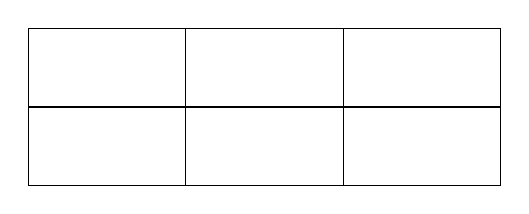
\begin{tikzpicture}
                \draw (0, 0) -- (2, 0) -- (2, 1) -- (0, 1) -- cycle;
                \draw (0, 1) -- (2, 1) -- (2, 2) -- (0, 2) -- cycle;
                \draw (2, 0) -- (4, 0) -- (4, 1) -- (2, 1) -- cycle;
                \draw (2, 1) -- (4, 1) -- (4, 2) -- (2, 2) -- cycle;
                \draw (4, 0) -- (6, 0) -- (6, 1) -- (4, 1) -- cycle;
                \draw (4, 1) -- (6, 1) -- (6, 2) -- (4, 2) -- cycle;
            \end{tikzpicture}
        \end{center}
        \vspace{3cm}
        \item Every student who applied for admission to a veterinary school has at least one
        pet: 30 have a cat, 28 have a dog, and 26 have fish. If 13 students have a fish and a
        cat, 15 students have fish and a dog, 11 students have both a cat and a dog, and 4
        students have a cat, a dog, and a fish, how many students applied to veterinary school?
        \begin{center}
            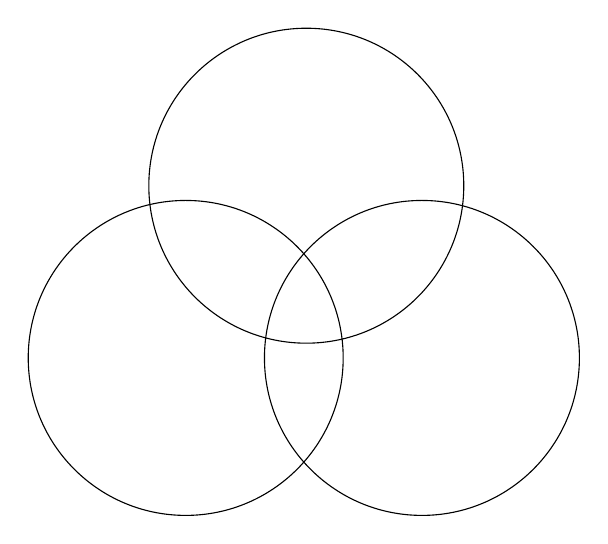
\begin{tikzpicture}
                \draw \firstcircle;
                \draw \secondcircle;
                \draw \thirdcircle;
            \end{tikzpicture}
        \end{center}
        \vspace{3cm}
    \end{enumerate}
\end{document}